% EMNLP 2026 - Compositional Skill Routing for LLM Agents
% Using ACL Rolling Review (ARR) format
\documentclass[11pt]{article}

% ARR / EMNLP 2026 style
\usepackage[hyperref]{acl}  % ACL Rolling Review style
\usepackage{times}
\usepackage{latexsym}
\usepackage{amsmath}
\usepackage{amssymb}
\usepackage{graphicx}
\usepackage{booktabs}
\usepackage{multirow}
\usepackage{xcolor}
\usepackage{enumitem}
\usepackage{url}
\usepackage{algorithm}
\usepackage{algorithmic}
\usepackage{subcaption}
\usepackage{tikz}
\usetikzlibrary{arrows.meta, positioning, shapes.geometric, fit, backgrounds}

% Custom commands
\newcommand{\system}{\textsc{SkillWeaver}}
\newcommand{\benchmark}{\textsc{CompSkillBench}}
\newcommand{\catrecall}{\text{CatR}}
\newcommand{\chaincat}{\text{Chain}_\text{cat}}

\title{Compositional Skill Routing for LLM Agents:\\Decompose, Retrieve, and Compose}

% Anonymous for review
\author{Anonymous}

\begin{document}
\maketitle

\begin{abstract}
LLM agents increasingly rely on external skills---reusable tool specifications---but real-world tasks often require \emph{composing} multiple skills, not just selecting one.
We formalize \textbf{Compositional Skill Routing}: given a complex query and a large skill library, decompose the query into atomic sub-tasks, retrieve the appropriate skill for each, and compose an executable plan.
We present \system{}, a decompose-retrieve-compose framework combining an LLM task decomposer, a bi-encoder skill retriever with FAISS indexing, and a dependency-aware DAG planner.
On \benchmark{}, a new benchmark of 300 compositional queries over 2{,}595 skills spanning 17 categories, we show that \emph{decomposition quality is the primary bottleneck}: oracle sub-tasks yield 99.5\% retrieval recall, while LLM decomposition reaches only 33.9\% category recall.
Our proposed \emph{Skill-Aware Decomposition} (SAD) closes this gap by feeding retrieved skill hints back to the decomposer, improving category recall to 54.2\% (+60\%) consistently across five models (7--72B); notably, a 7B model with SAD outperforms a 72B model without it.
\system{} further reduces context window consumption by over 99\% compared to exposing all tools.
\end{abstract}

% ============================================================
\section{Introduction}
\label{sec:intro}

The agent paradigm for large language models (LLMs) has evolved beyond single-turn generation to encompass tool use, planning, and multi-step task execution \cite{schick2023toolformer,qin2023toolllm,patil2023gorilla}.
A key architectural pattern emerging in modern LLM agents is the use of \emph{skills}: modular, reusable tool specifications that define specific capabilities along with instructions for when and how to invoke them \cite{anthropic2025skills}.
As agent skill libraries grow---with repositories already containing thousands of community-contributed skills---a fundamental routing question arises: \emph{given a user query, which skill(s) should the agent invoke?}

Prior work has largely treated skill routing as a single-skill selection problem, where the goal is to match a query to the single best skill \cite{xu2025skillrouter}.
However, real-world user queries frequently require \emph{multiple} skills working together.
For example, the query ``\textit{Download the dataset, transform it, and create visual reports}'' requires at least three distinct skills: an API client for downloading, a data processor for transformation, and a visualization tool for report generation.

We formalize this as the \textbf{Compositional Skill Routing} problem (Figure~\ref{fig:overview}):
given a complex query $q$ and a skill library $\mathcal{S}$, produce an ordered sequence of skills $[s_1, s_2, \ldots, s_k]$ that collectively accomplish the query, where each $s_i$ handles one atomic sub-task.
This formulation captures the compositional nature of real-world tasks while maintaining the modularity benefits of skill-based architectures.

We present \system{}, a three-stage framework that addresses this problem through:
\begin{enumerate}[nosep,leftmargin=*]
  \item \textbf{Decompose}: An LLM-based task decomposer that breaks complex queries into atomic sub-tasks, each requiring exactly one skill.
  \item \textbf{Retrieve}: A bi-encoder retriever that identifies candidate skills for each sub-task using semantic similarity over skill metadata.
  \item \textbf{Compose}: A compatibility-aware planner that selects the best skill per step while considering inter-skill compatibility, producing an executable DAG.
\end{enumerate}

To evaluate compositional skill routing, we construct \benchmark{}, the first dedicated benchmark for this task.
\benchmark{} contains 300 compositional queries over 2{,}595 curated skills spanning 17 functional categories, with ground-truth skill chains and three difficulty levels.
Skills are sourced from 212 public GitHub repositories and deduplicated to ensure quality.

Our experiments yield several key findings:
\begin{itemize}[nosep,leftmargin=*]
  \item \textbf{Decomposition is the bottleneck}: With oracle decomposition, our retriever achieves 99.5\% Recall@1 and perfect category accuracy. Standard LLM decomposition drops to 33.9\% $\catrecall$@1, identifying decomposition as the critical frontier.
  \item \textbf{Skill-aware decomposition closes the gap}: Our proposed \emph{Skill-Aware Decomposition} (SAD), which provides the decomposer with retrieved skill context, improves $\catrecall$@1 from 33.9\% to 54.2\% (+60\%) without changing the underlying model.
  \item \textbf{Metadata suffices for retrieval}: Metadata-only encoding matches or outperforms body-aware encoding, suggesting concise skill metadata carries the most discriminative signal.
\end{itemize}

\begin{figure*}[t]
\centering
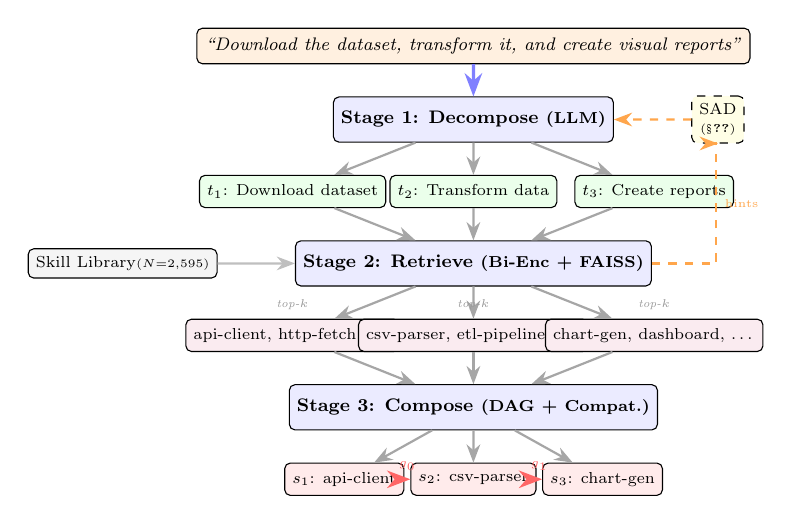
\begin{tikzpicture}[scale=0.82, every node/.append style={transform shape},
    >=Stealth,
    node distance=0.35cm and 0.5cm,
    stage/.style={draw, rounded corners=2pt, fill=blue!8, minimum height=0.7cm, minimum width=2.4cm, font=\footnotesize\bfseries, align=center},
    query/.style={draw, rounded corners=2pt, fill=orange!12, minimum height=0.55cm, font=\footnotesize, align=center},
    subtask/.style={draw, rounded corners=2pt, fill=green!8, minimum height=0.5cm, font=\scriptsize, align=center},
    skill/.style={draw, rounded corners=2pt, fill=purple!8, minimum height=0.5cm, font=\scriptsize, align=center},
    dag/.style={draw, rounded corners=2pt, fill=red!8, minimum height=0.5cm, font=\scriptsize, align=center},
    arrow/.style={->, thick, color=gray!70},
    bigarrow/.style={->, very thick, color=blue!50},
    lbl/.style={font=\tiny\itshape, color=gray!80},
]
\node[query, minimum width=6cm] (query) {\textit{``Download the dataset, transform it, and create visual reports''}};
\node[stage, below=0.5cm of query] (stage1) {Stage 1: Decompose {\scriptsize (LLM)}};
\draw[bigarrow] (query) -- (stage1);
\node[subtask, below=0.5cm of stage1, xshift=-2.8cm] (t1) {$t_1$: Download dataset};
\node[subtask, below=0.5cm of stage1] (t2) {$t_2$: Transform data};
\node[subtask, below=0.5cm of stage1, xshift=2.8cm] (t3) {$t_3$: Create reports};
\draw[arrow] (stage1) -- (t1); \draw[arrow] (stage1) -- (t2); \draw[arrow] (stage1) -- (t3);
\node[stage, below=0.5cm of t2] (stage2) {Stage 2: Retrieve {\scriptsize (Bi-Enc + FAISS)}};
\draw[arrow] (t1) -- (stage2); \draw[arrow] (t2) -- (stage2); \draw[arrow] (t3) -- (stage2);
\node[skill, below=0.5cm of stage2, xshift=-2.8cm] (c1) {api-client, http-fetch, \ldots};
\node[skill, below=0.5cm of stage2] (c2) {csv-parser, etl-pipeline, \ldots};
\node[skill, below=0.5cm of stage2, xshift=2.8cm] (c3) {chart-gen, dashboard, \ldots};
\draw[arrow] (stage2) -- (c1); \draw[arrow] (stage2) -- (c2); \draw[arrow] (stage2) -- (c3);
\node[lbl, above=0.02cm of c1] {top-$k$}; \node[lbl, above=0.02cm of c2] {top-$k$}; \node[lbl, above=0.02cm of c3] {top-$k$};
\node[stage, below=0.5cm of c2] (stage3) {Stage 3: Compose {\scriptsize (DAG + Compat.)}};
\draw[arrow] (c1) -- (stage3); \draw[arrow] (c2) -- (stage3); \draw[arrow] (c3) -- (stage3);
\node[dag, below=0.5cm of stage3, xshift=-2cm] (s1) {$s_1$: api-client};
\node[dag, below=0.5cm of stage3] (s2) {$s_2$: csv-parser};
\node[dag, below=0.5cm of stage3, xshift=2cm] (s3) {$s_3$: chart-gen};
\draw[arrow] (stage3) -- (s1); \draw[arrow] (stage3) -- (s2); \draw[arrow] (stage3) -- (s3);
\draw[->, very thick, color=red!60] (s1) -- node[above, font=\tiny] {$g_0$} (s2);
\draw[->, very thick, color=red!60] (s2) -- node[above, font=\tiny] {$g_1$} (s3);
\node[draw, dashed, rounded corners=2pt, fill=yellow!10, minimum height=0.5cm, font=\scriptsize, align=center, right=1.2cm of stage1] (sad) {SAD\\{\tiny (\S\ref{sec:sad})}};
\draw[->, dashed, thick, color=orange!70] (stage2.east) -- ++(1.0,0) |- node[right, pos=0.25, font=\tiny, color=orange!70] {hints} (sad.south);
\draw[->, dashed, thick, color=orange!70] (sad.west) -- (stage1.east);
\node[draw, rounded corners=2pt, fill=gray!8, font=\scriptsize, minimum height=0.4cm, left=1.2cm of stage2] (lib) {Skill Library\\{\tiny ($N{=}2{,}595$)}};
\draw[arrow, color=gray!50] (lib) -- (stage2);
\end{tikzpicture}
\caption{Overview of \system{}. A query is decomposed into sub-tasks, each matched to skills via bi-encoder retrieval, then composed into a DAG. Dashed arrows: SAD feedback loop (\S\ref{sec:sad}).}
\label{fig:overview}
\end{figure*}

% ============================================================
\section{Related Work}
\label{sec:related}

\paragraph{Tool Selection and Routing.}
Tool selection for LLMs has been studied through API retrieval \cite{patil2023gorilla,qin2023toolllm}, tool documentation matching \cite{hao2024toolkengpt}, and hierarchical routing \cite{xu2025skillrouter}.
AnyTool \cite{du2024anytool} uses self-reflection to navigate hierarchical API pools, and CRAFT \cite{yuan2024craft} creates specialized toolsets per query via retrieval.
SkillRouter \cite{xu2025skillrouter} is closest to our work, introducing a bi-encoder approach for single-skill routing.
However, all these methods select tools independently per query; none jointly optimizes decomposition, retrieval, and inter-skill compatibility for compositional tasks.

\paragraph{Tool-Augmented LLM Benchmarks.}
Evaluating tool use has received growing attention.
API-Bank \cite{li2023apibank} and ToolQA \cite{zhuang2024toolqa} benchmark single-tool and multi-step tool use respectively.
ToolSandbox \cite{lu2024toolsandbox} provides a stateful evaluation framework, and MetaTool \cite{huang2024metatool} focuses on deciding \emph{whether} to use tools.
TaskBench \cite{shen2023taskbench} evaluates multi-step tasks but over a fixed set of tools rather than retrieval from a large library.
Our \benchmark{} is the first benchmark specifically designed for compositional \emph{routing} over thousands of skills.

\paragraph{Task Decomposition and Planning.}
LLM-based task decomposition has been explored through prompting strategies \cite{wei2022chain,zhou2022least,khot2023decomposed}, planning frameworks \cite{huang2022language,wang2023plan}, and agentic systems \cite{yao2023react,shinn2023reflexion}.
\citet{press2023measuring} identify a ``compositionality gap'' in language models, motivating decomposition-based approaches.
TPTU \cite{ruan2024tptu} and AgentFlan \cite{chen2024agentflan} study joint task planning and tool use.
Our work contributes a novel \emph{skill-aware} decomposition approach where the decomposer is informed by the skill library itself, creating a retrieval-augmented feedback loop.

\paragraph{Retrieval-Augmented Generation.}
Dense retrieval using bi-encoders \cite{karpukhin2020dense,ni2022sentence} has been widely applied to knowledge-intensive NLP tasks.
We adapt this paradigm for skill retrieval, and further extend it to inform the upstream decomposition stage---using retrieval results as decomposition guidance.

% ============================================================
\section{Problem Formulation}
\label{sec:problem}

\paragraph{Skill Library.}
A skill library $\mathcal{S} = \{s_1, \ldots, s_N\}$ contains $N$ skills.
Each skill $s_i$ is a tuple $(n_i, d_i, b_i, C_i)$ where $n_i$ is the name, $d_i$ is a natural language description, $b_i$ is the full specification body (instructions, examples, configuration), and $C_i \subseteq \mathcal{C}$ is a set of functional categories from a taxonomy $\mathcal{C}$.

\paragraph{Compositional Skill Routing.}
Given a complex query $q$ that requires multiple capabilities, the goal is to produce:
\begin{enumerate}[nosep,leftmargin=*]
  \item A decomposition $D(q) = [t_1, \ldots, t_K]$ of $K$ atomic sub-tasks.
  \item A skill assignment $\sigma: [t_1, \ldots, t_K] \to \mathcal{S}^K$ mapping each sub-task to a skill.
  \item An execution plan (DAG) $G = (V, E)$ specifying dependencies between steps.
\end{enumerate}

The compositional routing function is $f: q \to (D, \sigma, G)$ optimizing:
\begin{equation}
\max_{D, \sigma, G} \sum_{k=1}^{K} \text{rel}(t_k, \sigma(t_k)) + \lambda \!\!\!\sum_{(i,j) \in E}\!\!\! \text{compat}(\sigma_i, \sigma_j)
\end{equation}
where $\text{rel}(\cdot)$ measures sub-task--skill relevance and $\text{compat}(\cdot)$ measures inter-skill compatibility.

% ============================================================
\section{Method: \system{}}
\label{sec:method}

\system{} implements compositional skill routing through three cascaded stages (Figure~\ref{fig:overview}).

\subsection{Stage 1: Task Decomposition}

Given a complex query $q$, the task decomposer uses an instruction-tuned LLM to produce an ordered list of atomic sub-tasks:
\begin{equation}
D(q) = \text{LLM}(p_{\text{sys}}, p_{\text{user}}(q)) = [t_1, \ldots, t_K]
\end{equation}
where $p_{\text{sys}}$ is a system prompt that instructs the model to decompose queries into sub-tasks, each requiring exactly one skill.
The output is constrained to a JSON array of strings for reliable parsing.

We apply the model's native chat template (e.g., ChatML for Qwen models) to ensure proper instruction following.
A fallback parser handles cases where the LLM produces numbered lists or other non-JSON formats.

\subsection{Stage 2: Skill Retrieval}

For each sub-task $t_k$, we retrieve the top-$m$ candidate skills from the library using a bi-encoder architecture:
\begin{equation}
\text{cand}(t_k) = \text{top-}m_{s \in \mathcal{S}} \; \cos(E_q(t_k), E_s(s))
\end{equation}
where $E_q$ and $E_s$ are the query and skill encoders (shared parameters), implemented using BGE-large-en-v1.5 \cite{xiao2023bge}.

\paragraph{Skill Representation.}
We investigate two encoding strategies:
\begin{itemize}[nosep,leftmargin=*]
  \item \textbf{Metadata-only}: $\text{repr}(s) = n_s \oplus d_s$ (name and description)
  \item \textbf{Body-aware}: $\text{repr}(s) = n_s \oplus d_s \oplus b_s[:L]$ (with truncated body)
\end{itemize}
where $\oplus$ denotes concatenation and $L=2000$ characters.

Embeddings are $L_2$-normalized and indexed using FAISS \cite{johnson2019faiss} for efficient inner product search.

\subsection{Stage 3: Dependency-Aware DAG Planning}
\label{sec:compose}

Unlike prior work that assumes a fixed sequential execution order, \system{} infers task dependencies and identifies parallelizable sub-tasks, producing a \emph{directed acyclic graph} (DAG) as the execution plan.

\paragraph{Dependency Detection.}
Given subtasks $[t_1, \ldots, t_K]$, we detect pairwise dependencies using three complementary signals:
\begin{enumerate}[nosep,leftmargin=*]
  \item \textbf{I/O type overlap}: If the expected output types of $t_i$ intersect with the required input types of $t_j$, we infer $t_i \to t_j$.
  \item \textbf{Producer--consumer patterns}: Curated keyword sets identify output-producing actions (\emph{generate, fetch, extract}) and input-consuming actions (\emph{parse, analyze, deploy}). If $t_i$ matches a producer pattern and $t_j$ a consumer, we infer a dependency.
  \item \textbf{Linguistic markers}: Phrases such as ``\emph{then},'' ``\emph{after},'' ``\emph{based on}'' in $t_j$'s description signal explicit dependency on a prior step.
\end{enumerate}
If no dependencies are detected, the planner conservatively falls back to sequential chaining.

\paragraph{Parallel Group Assignment.}
Given dependency edges $E$, we assign each sub-task to a parallel group $g(t_k)$ via topological level assignment (Kahn's algorithm):
\begin{equation}
g(t_k) = \begin{cases} 0 & \text{if } \text{indeg}(t_k) = 0 \\ \max_{(t_i, t_k) \in E}\; g(t_i) + 1 & \text{otherwise} \end{cases}
\label{eq:parallel}
\end{equation}
Sub-tasks with the same group number have no mutual dependencies and can execute concurrently, reducing the critical-path length from $K$ (fully sequential) to the DAG depth $d \leq K$.

\paragraph{Multi-Dimensional Compatibility.}
We define a four-dimensional compatibility function between upstream skill $s_a$ and downstream candidate $s_b$:
\begin{equation}
\text{compat}(s_a, s_b) = \sum_{d \in \mathcal{D}} w_d \cdot \phi_d(s_a, s_b)
\label{eq:compat}
\end{equation}
where $\mathcal{D} = \{\text{io}, \text{cat}, \text{tag}, \text{kw}\}$: $\phi_\text{io}$ measures I/O type compatibility via a type coercion matrix; $\phi_\text{cat}$ and $\phi_\text{tag}$ compute Jaccard similarity over categories and tags; $\phi_\text{kw}$ detects producer--consumer keyword co-occurrence. We set weights $(0.4, 0.2, 0.2, 0.2)$.

\paragraph{DAG-Aware Skill Selection.}
The final skill per step combines retrieval relevance with DAG-predecessor compatibility:
\begin{equation}
\sigma(t_k) = \arg\max_{s \in \text{cand}(t_k)} \alpha \!\cdot\! \text{sim}(t_k, s) + (1\!-\!\alpha) \!\cdot\! \bar{c}_k(s)
\end{equation}
where $\bar{c}_k(s) = |\text{pred}(k)|^{-1}\!\sum_{i \in \text{pred}(k)} \text{compat}(\sigma_i, s)$ averages compatibility with all DAG predecessors.

\subsection{Skill-Aware Decomposition (SAD)}
\label{sec:sad}

A key finding from our experiments (\S\ref{sec:results}) is that the decomposition stage is the primary bottleneck.
Standard LLM decomposition generates sub-task descriptions using only the query, often producing generic phrasings that misalign with the skill vocabulary.

We propose \emph{Skill-Aware Decomposition} (SAD), which augments the decomposer's input with preliminary skill library information.
Given query $q$, we first perform a preliminary retrieval over the full skill library to obtain the top-$H$ candidate skills, then provide their names, categories, and truncated descriptions as hints in the decomposition prompt:
\begin{equation}
D_{\text{SAD}}(q) = \text{LLM}(p_{\text{sys}}(\text{hints}(q, H)), p_{\text{user}}(q))
\label{eq:sad}
\end{equation}
where $\text{hints}(q, H) = \{(n_s, c_s, d_s[:120]) \mid s \in \text{top-}H(q)\}$.
This creates a retrieval-augmented feedback loop: the skill library informs decomposition, which produces sub-tasks better aligned with the skill vocabulary, improving downstream retrieval.
SAD requires no additional training---it modifies only the decomposition prompt.


% ============================================================
\section{Benchmark: \benchmark{}}
\label{sec:benchmark}

\subsection{Skill Pool Construction}

We collect skills from 212 public GitHub repositories that adopt the SKILL.md specification format \cite{anthropic2025skills}.
The raw collection yields 11{,}011 skills.
We apply the following curation pipeline:

\begin{enumerate}[nosep,leftmargin=*]
  \item \textbf{Deduplication}: Skills with identical names are merged, reducing to 7{,}681 unique skills.
  \item \textbf{Quality filtering}: Skills without descriptions or with descriptions shorter than 10 characters are removed.
  \item \textbf{Categorization}: Skills are assigned to 17 functional categories (Table~\ref{tab:categories}) using keyword matching on name and description fields only.
  Anti-keywords prevent false positive assignments (e.g., ``debug'' skills are excluded from ``deployment'').
  Skills matching no category or multiple conflicting categories are excluded.
  \item The final pool contains \textbf{2{,}595} categorized skills.
\end{enumerate}

\begin{table}[t]
\centering
\small
\setlength{\tabcolsep}{4pt}
\begin{tabular}{lrl}
\toprule
\textbf{Category} & \textbf{Count} & \textbf{Examples} \\
\midrule
Code Generator & 389 & prd-generator, nextjs-dev \\
API Client & 312 & stripe-api, github-api \\
Test Writer & 248 & unit-test-gen, qa-suite \\
Data Processor & 221 & csv-parser, etl-pipeline \\
Code Analyzer & 187 & code-review, lint-checker \\
Writer & 176 & blog-writer, doc-gen \\
Deployment & 142 & k8s-deploy, ci-cd-setup \\
Security & 118 & vuln-scanner, audit-tool \\
Visualizer & 97 & chart-gen, dashboard-builder \\
Search & 96 & web-search, code-search \\
\midrule
\multicolumn{2}{l}{\textit{+ 7 more categories}} & 609 total \\
\bottomrule
\end{tabular}
\caption{Top 10 skill categories in \benchmark{} (of 17 total). The full pool contains 2{,}595 skills from 212 repositories.}
\label{tab:categories}
\end{table}

\subsection{Query Generation}
\label{sec:querygen}

Compositional queries are generated programmatically by combining skills from different categories into multi-step tasks.
For each query, the generation pipeline: (1)~samples $K$ skill categories according to the target difficulty level, (2)~selects one skill per category from the pool, (3)~constructs a natural language query by concatenating action-verb templates with the selected skill descriptions, and (4)~records the selected skill IDs and their descriptions as ground-truth sub-tasks.

\paragraph{Difficulty Levels.}
\begin{itemize}[nosep,leftmargin=*]
  \item \textbf{Easy} (117 queries): 2 skills, 2 categories
  \item \textbf{Medium} (120 queries): 3 skills, 3 categories
  \item \textbf{Hard} (63 queries): 4--5 skills, 4--5 categories
\end{itemize}

Each query is associated with ground-truth sub-task descriptions (derived from actual skill descriptions), ground-truth skill IDs, required categories, and a sequential execution order.
The benchmark totals 300 queries involving 523 unique ground-truth skills.

\paragraph{Text Overlap Disclosure.}
Because ground-truth sub-task descriptions are derived from skill metadata, there is substantial lexical overlap between sub-task descriptions and skill descriptions in the library.
An automated analysis reveals mean ROUGE-L of 0.845 and mean BLEU-1 of 0.980 between ground-truth sub-tasks and their corresponding skill descriptions, with 37.8\% being exact copies.
This explains the near-perfect oracle retrieval performance (R@1 = 99.5\%) and means that absolute retrieval scores on template queries should be interpreted as upper-bound estimates.
Our human-written query evaluation (\S\ref{sec:sad-results}) provides a complementary assessment with naturalistic phrasing diversity, where performance drops substantially (e.g., $\catrecall$@1: 25.9\% vs 54.2\%), confirming that template-based scores overestimate real-world performance.

\subsection{Evaluation Metrics}

We evaluate at three granularities:

\paragraph{Step-Level Metrics.}
\begin{itemize}[nosep,leftmargin=*]
  \item \textbf{Skill Recall@$k$} (R@$k$): Fraction of steps where the ground-truth skill appears in the top-$k$ candidates.
  \item \textbf{Category Recall@$k$} ($\catrecall$@$k$): Fraction of steps where \emph{any skill from the correct category} appears in the top-$k$.
  This relaxed metric is more practical, as many skills within a category are functionally interchangeable.
\end{itemize}

\paragraph{Chain-Level Metrics.}
\begin{itemize}[nosep,leftmargin=*]
  \item \textbf{Chain Exact Match}: Fraction of queries where \emph{all} steps select the exact ground-truth skill.
  \item \textbf{Chain Category Match} ($\chaincat$): Average fraction of steps per query that select a skill from the correct category.
\end{itemize}

\paragraph{Decomposition Accuracy.} Fraction of queries where the predicted number of sub-tasks matches the ground truth.

% ============================================================
\section{Experimental Setup}
\label{sec:setup}

\paragraph{LLM Decomposers.}
We compare five open-weight instruction-tuned models spanning three scales:
Qwen2.5-7B-Instruct, Qwen2.5-14B-Instruct, and Qwen2.5-72B-Instruct \cite{qwen2.5}, 
Llama-3.1-8B-Instruct \cite{dubey2024llama3}, and 
Mistral-7B-Instruct-v0.3 \cite{jiang2023mistral}.
Generation uses temperature $\tau=0.1$, $\text{top}_p=0.9$, and a maximum of 256 new tokens.

\paragraph{Retriever.}
BGE-large-en-v1.5 \cite{xiao2023bge} (1024-dim) serves as the bi-encoder, with FAISS IndexFlatIP for exact inner product search.
We set $k=10$ for retrieval unless otherwise noted.

\paragraph{Baselines.}
\begin{itemize}[nosep,leftmargin=*]
  \item \textbf{Single-Skill}: No decomposition; the full query is used to retrieve one skill set applied to all steps. This represents current single-skill routing methods.
  \item \textbf{Oracle Decomposition}: Ground-truth sub-task descriptions are used for retrieval, establishing an upper bound on decomposition quality.
\end{itemize}

\paragraph{Hardware.} 
7--14B models run on a single NVIDIA A100-80GB GPU.
The 72B model uses four A100-80GB GPUs with automatic tensor parallelism via \texttt{device\_map="auto"}.

% ============================================================
\section{Results}
\label{sec:results}

\subsection{Main Results}

Table~\ref{tab:main} presents the main experimental results across all configurations.

\begin{table*}[t]
\centering
\small
\resizebox{\textwidth}{!}{
\begin{tabular}{llccccccc}
\toprule
\textbf{Method} & \textbf{Signal} & \textbf{Decomp\%} & \textbf{R@1} & \textbf{R@10} & $\catrecall$\textbf{@1} & $\catrecall$\textbf{@10} & \textbf{Chain}$_E$ & $\chaincat$ \\
\midrule
\multicolumn{9}{l}{\textit{Baselines}} \\
Single-Skill & Meta & -- & 0.000 & 0.029 & 0.211 & 0.698 & 0.000 & 0.216 \\
Single-Skill & Body & -- & 0.002 & 0.028 & 0.285 & 0.633 & 0.000 & 0.293 \\
Oracle Decomp & Meta & 1.000 & \textbf{0.995} & \textbf{1.000} & \textbf{1.000} & \textbf{1.000} & \textbf{0.987} & \textbf{1.000} \\
Oracle Decomp & Body & 1.000 & 0.990 & 1.000 & 0.998 & 1.000 & 0.970 & 0.998 \\
\midrule
\multicolumn{9}{l}{\textit{Full Pipeline (\system{})}} \\
Qwen2.5-7B & Meta & 0.360 & 0.005 & 0.034 & 0.339 & 0.649 & 0.000 & 0.316 \\
Qwen2.5-7B & Body & 0.370 & 0.008 & 0.029 & \underline{0.363} & \underline{0.662} & 0.000 & \underline{0.345} \\
Llama-3.1-8B & Meta & 0.000 & 0.002 & 0.016 & 0.216 & 0.507 & 0.000 & 0.210 \\
Mistral-7B & Meta & 0.177 & 0.005 & 0.036 & 0.243 & 0.607 & 0.000 & 0.248 \\
\bottomrule
\end{tabular}
}
\caption{Main results on \benchmark{}. \textbf{Bold}: best overall. \underline{Underline}: best among full pipeline configurations. R@$k$: Skill Recall@$k$. $\catrecall$@$k$: Category Recall@$k$. Chain$_E$: Chain Exact Match. $\chaincat$: Chain Category Match. Decomp\%: decomposition accuracy (correct number of sub-tasks).}
\label{tab:main}
\end{table*}

\paragraph{Decomposition is the bottleneck.}
Oracle decomposition achieves R@1 = 99.5\% and perfect category accuracy.
The best LLM decomposer (Qwen2.5-7B) reaches only $\catrecall$@1 = 36.3\%, confirming decomposition quality as the primary bottleneck.

\paragraph{Compositional routing outperforms single-skill.}
Our full pipeline achieves $\catrecall$@1 = 33.9\%, substantially outperforming the single-skill baseline (21.1\%), validating that even approximate decomposition aids compositional routing.

\paragraph{Metadata matches or outperforms body.}
Metadata-only retrieval achieves oracle R@1 = 99.5\% vs 99.0\% for body-aware.
In the full pipeline, body-aware has a slight edge ($\catrecall$@1: 36.3\% vs 33.9\%) but with higher encoding cost, suggesting concise metadata captures the essential discriminative signal.

\subsection{Decomposer Comparison}

\begin{table}[t]
\centering
\small
\begin{tabular}{lccc}
\toprule
\textbf{Decomposer} & \textbf{Decomp\%} & $\catrecall$\textbf{@1} & $\chaincat$ \\
\midrule
Qwen2.5-7B & \textbf{0.360} & \textbf{0.339} & \textbf{0.316} \\
Mistral-7B & 0.177 & 0.243 & 0.248 \\
Llama-3.1-8B & 0.000 & 0.216 & 0.210 \\
\midrule
Oracle & 1.000 & 1.000 & 1.000 \\
\bottomrule
\end{tabular}
\caption{Decomposer comparison (all using metadata-only retrieval). Qwen2.5-7B achieves the best decomposition accuracy and downstream routing performance.}
\label{tab:decomposer}
\end{table}

Table~\ref{tab:decomposer} compares the three LLM decomposers.
Qwen2.5-7B significantly outperforms the other models, achieving 36.0\% decomposition accuracy versus 17.7\% for Mistral and 0\% for Llama.

\paragraph{Over-decomposition is the primary failure mode.}
Analysis of decomposition patterns (Figure~\ref{fig:decomp_dist}) reveals that Llama-3.1-8B systematically over-decomposes: its median output is 9 sub-tasks, while the ground truth distribution peaks at 2--3.
No single Llama decomposition matches the ground-truth count, explaining its 0\% decomposition accuracy.
Mistral shows a similar but less severe tendency, while Qwen's distribution most closely aligns with the ground truth.

\subsection{Difficulty Analysis}

\begin{table}[t]
\centering
\small
\begin{tabular}{llccc}
\toprule
\textbf{Method} & \textbf{Diff.} & $\catrecall$\textbf{@1} & $\catrecall$\textbf{@10} \\
\midrule
\multirow{3}{*}{Single-Skill} & Easy & 0.201 & 0.774 \\
& Medium & 0.267 & 0.667 \\
& Hard & 0.146 & 0.675 \\
\midrule
\multirow{3}{*}{Qwen + Meta} & Easy & 0.214 & 0.637 \\
& Medium & 0.367 & 0.658 \\
& Hard & \textbf{0.410} & 0.646 \\
\midrule
\multirow{3}{*}{Qwen + Body} & Easy & 0.252 & 0.607 \\
& Medium & \textbf{0.403} & \textbf{0.728} \\
& Hard & 0.407 & 0.623 \\
\bottomrule
\end{tabular}
\caption{Performance by difficulty level. Decomposition-based routing shows increasing advantage on harder queries.}
\label{tab:difficulty}
\end{table}

Table~\ref{tab:difficulty} breaks down results by difficulty level.
The decomposition-based pipeline shows its \emph{greatest advantage on harder queries}: for hard queries (4--5 skills), Qwen + Meta achieves $\catrecall$@1 = 41.0\% versus the single-skill baseline at 14.6\% (+181\%).
This pattern suggests that decomposition becomes increasingly important as task complexity grows.

\subsection{Skill-Aware Decomposition Results}
\label{sec:sad-results}

\begin{table}[t]
\centering
\small
\begin{tabular}{lccc}
\toprule
\textbf{Configuration} & \textbf{DA} & \textbf{CatR@1} & \textbf{ChainCat} \\
\midrule
Vanilla (no hints) & 0.360 & 0.339 & 0.316 \\
\midrule
SAD ($H{=}5$) & 0.607 & 0.389 & 0.326 \\
SAD ($H{=}10$) & 0.657 & 0.481 & 0.466 \\
SAD ($H{=}15$) & \textbf{0.687} & \textbf{0.542} & \textbf{0.516} \\
SAD ($H{=}25$) & 0.790 & 0.474 & 0.471 \\
\bottomrule
\end{tabular}
\caption{Ablation over the number of skill hints $H$ for SAD with Qwen2.5-7B. DA increases monotonically with $H$, but CatR@1 peaks at $H{=}15$, indicating a noise--alignment trade-off.}
\label{tab:sad-ablation}
\end{table}

Table~\ref{tab:sad-ablation} presents the ablation over hint count $H$.
DA increases monotonically (36.0\% to 79.0\%), but $\catrecall$@1 peaks at $H{=}15$ (54.2\%) before declining at $H{=}25$ (47.4\%), revealing a noise--alignment trade-off.

\begin{table}[t]
\centering
\small
\begin{tabular}{llccc}
\toprule
\textbf{Model} & \textbf{Method} & \textbf{DA} & \textbf{CatR@1} & $\chaincat$ \\
\midrule
\multirow{2}{*}{Qwen2.5-7B} & Vanilla & 0.360 & 0.339 & 0.316 \\
 & +SAD & \textbf{0.687} & \textbf{0.542} & \textbf{0.516} \\
\midrule
\multirow{2}{*}{Qwen2.5-14B} & Vanilla & 0.280 & 0.297 & 0.280 \\
 & +SAD & 0.447 & 0.399 & 0.320 \\
\midrule
\multirow{2}{*}{Llama-3.1-8B} & Vanilla & 0.000 & 0.216 & 0.210 \\
 & +SAD & 0.107 & 0.339 & 0.359 \\
\midrule
\multirow{2}{*}{Mistral-7B} & Vanilla & 0.177 & 0.242 & 0.248 \\
 & +SAD & 0.273 & 0.307 & 0.301 \\
\midrule
\multirow{2}{*}{Qwen2.5-72B} & Vanilla & 0.627 & 0.368 & 0.358 \\
 & +SAD & 0.503 & 0.483 & \underline{0.518} \\
\bottomrule
\end{tabular}
\caption{Cross-model SAD ($H{=}15$). SAD improves routing across five models (7--72B). \textbf{Bold}: best. \underline{Underline}: second best. 7B+SAD surpasses the 10$\times$ larger 72B vanilla.}
\label{tab:sad-crossmodel}
\end{table}

Table~\ref{tab:sad-crossmodel} shows SAD generalizes across model families, with $\catrecall$@1 gains from +26.9\% (Mistral) to +59.9\% (Qwen-7B).
\textbf{Qwen2.5-7B+SAD (54.2\%) outperforms 72B vanilla (36.8\%)}, showing retrieval-augmented decomposition can surpass a 10$\times$ larger model.
The 72B model's SAD reduces DA from 62.7\% to 50.3\% while improving $\catrecall$@1 to 48.3\%, suggesting SAD restructures outputs toward skill-aligned phrasing.
The 14B anomaly (lower performance than 7B) stems from over-decomposition and lower JSON parse rates; see Appendix~\ref{app:14b}.

\paragraph{Human-written query generalization.}
On 55 human-written queries (22 easy, 23 medium, 10 hard), SAD improves $\catrecall$@1 from 18.8\% to 30.8\% (+63.8\%).
Hard queries decline (17.0\% $\to$ 9.4\%), suggesting hints become overwhelming for complex decompositions.
The lower absolute numbers confirm human phrasing diversity remains challenging.

\subsection{Context Window Analysis}
\label{sec:context}

Table~\ref{tab:context} quantifies context savings: exposing all 2{,}595 skills consumes $\sim$1.04M tokens, exceeding most LLM contexts; \system{} reduces this to 2--5 skills per query ($>$99\% reduction).

\begin{table}[t]
\centering
\small
\begin{tabular}{@{}lrrr@{}}
\toprule
\textbf{Strategy} & \textbf{Tools} & \textbf{Est.\ Tokens} & \textbf{Reduction} \\
\midrule
All tools (na\"ive) & 2{,}595 & $\sim$1{,}038K & --- \\
Top-$k$ flat retrieval & 10 & $\sim$4{,}000 & 99.6\% \\
\system{} (avg.\ chain) & 2.9 & $\sim$1{,}160 & 99.9\% \\
\bottomrule
\end{tabular}
\caption{Context window consumption (${\sim}$400 tokens/tool). Compositional routing reduces consumption by two orders of magnitude.}
\label{tab:context}
\end{table}

% ============================================================
\section{Analysis}
\label{sec:analysis}

\subsection{Error Analysis}

We examine 50 failure cases from the Qwen + Meta pipeline.
\textbf{Over-decomposition} (36\%) inserts unnecessary intermediate steps;
\textbf{generic descriptions} (28\%) produce overly broad phrasings that misalign with skills;
\textbf{vocabulary mismatch} (22\%) uses different terminology than skill metadata;
\textbf{under-decomposition} (14\%) merges multiple steps, typically for 4+ skill queries.

\subsection{Case Study and Oracle Retrieval}

``\textit{Generate code, write tests, deploy}'' correctly decomposes into three ground-truth-matching sub-tasks.
Conversely, ``\textit{Draft and localize a document}'' (2 skills) yields 7 sub-tasks---a typical over-decomposition failure.
Oracle R@1 (99.5\%) confirms retriever quality; the 0.5\% failures occur when skills share near-identical metadata.

% ============================================================
\section{Discussion}
\label{sec:discussion}

\paragraph{The decomposition gap.}
Standard 7B decomposition yields $\catrecall$@1 = 33.9\%, a 66-point gap from oracle.
Scaling to 72B improves this to only 36.8\%, confirming that model size alone is insufficient.
SAD narrows the gap to 46 points ($\catrecall$@1 = 54.2\% with 7B+SAD): \textbf{7B+SAD surpasses 72B vanilla by 7.4 points} while using $10\times$ fewer parameters.
The hint count ablation reveals a noise--alignment trade-off (DA increases monotonically, but retrieval peaks at $H{=}15$).
Cross-model results across five models (7B--72B) confirm SAD as a model-agnostic improvement.

\paragraph{Metadata vs.\ body.}
Metadata-only retrieval matches body-aware encoding, contrasting with \citet{xu2025skillrouter}'s finding that body content is ``decisive'' for single-skill routing.
We hypothesize that compositional decomposition produces targeted sub-task queries that align naturally with concise metadata.

\paragraph{Scalability and planning.}
FAISS retrieval scales to thousands of skills; end-to-end median latency is 568ms (p95: 1.26s).
Our DAG planner achieves 80.0\% edge detection on a 20-query pilot.
We define \emph{functional coherence} as the fraction of adjacent skill pairs with compatible I/O categories (53.7\% on pilot).
Compositional routing reduces context consumption by over 99\% (\S\ref{sec:context}).

% ============================================================
\section{Conclusion}
\label{sec:conclusion}

We formalized Compositional Skill Routing and presented \system{}, a decompose-retrieve-compose framework.
SAD improves decomposition accuracy from 36\% to 69\% and $\catrecall$@1 by 60\% across five models (7--72B)---a 7B model with SAD outperforms a 72B model without it.
On \benchmark{} (300 queries, 2{,}595 skills), oracle decomposition achieves near-perfect retrieval, identifying decomposition as the primary bottleneck.
Over-decomposition and vocabulary mismatch are the dominant failure modes, pointing to decomposition-aware training as the most promising future direction.

% ============================================================
\section*{Limitations}

Our benchmark uses template-based query generation with high text overlap (ROUGE-L=0.845); while 55 human-written queries show consistent SAD gains on easy/medium difficulties, hard queries (4--5 skills) see performance decline.
The DAG planner's parallelization capability lacks partial-order ground-truth evaluation.
Our evaluation is retrieval-focused; full end-to-end evaluation with actual skill execution and learning-based dependency prediction remain future work.

\section*{Ethics Statement}

This work uses only publicly available, open-source skill repositories and involves no human subjects or personal data.
We encourage responsible deployment of skill routing systems with human oversight.

% ============================================================
% References
\bibliography{references}

% ============================================================
\appendix

\section{Category Taxonomy}
\label{app:categories}

The 17 functional categories in \benchmark{} are: 
code\_generator, api\_client, test\_writer, data\_processor, code\_analyzer, writer, deployment, security, visualizer, search, refactorer, file\_converter, translator, database, monitoring, designer, git\_workflow.

\section{Decomposition Distribution}
\label{app:decomp}

Figure~\ref{fig:decomp_dist} shows the distribution of predicted sub-task counts for each LLM decomposer compared to the ground truth.

\begin{figure}[h]
\centering
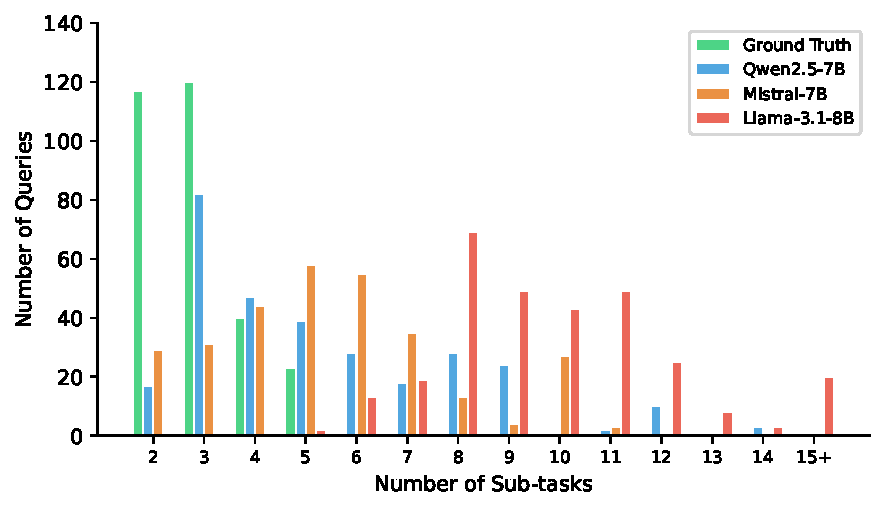
\includegraphics[width=\columnwidth]{figures/decomp_dist.pdf}
\caption{Distribution of predicted sub-task counts by decomposer. Llama-3.1-8B systematically over-decomposes (median 9 sub-tasks), while Qwen2.5-7B most closely aligns with the ground truth distribution (peak at 2--3).}
\label{fig:decomp_dist}
\end{figure}

\section{Top-$k$ Sensitivity}
\label{app:topk}

With oracle decomposition, R@1 = 99.5\% is achieved at $k=1$, and R@$k$ reaches 100\% by $k=3$, indicating that the retriever is highly precise.

\section{14B Anomaly Analysis}
\label{app:14b}

The counter-intuitive result that Qwen2.5-14B underperforms the 7B variant warrants further examination.
Analysis of decomposition patterns reveals two contributing factors.
First, 14B vanilla produces an average of 5.3 sub-tasks per query (vs.\ 2.9 for 7B), with 42.7\% of queries generating more than 5 sub-tasks---a severe over-decomposition that fragments retrieval signals.
Second, only 71.3\% of 14B vanilla outputs parse as valid JSON (vs.\ 89.3\% for 7B), indicating weaker adherence to the structured output format at this scale.
With SAD, the 14B model's JSON parse rate improves to 85.0\%, but 44.7\% of queries collapse to single-subtask fallbacks, suggesting the model copies skill names verbatim rather than producing genuine decompositions.
These findings indicate that larger models are not uniformly better at structured decomposition, and that instruction-following for constrained output formats is a distinct capability from general language understanding.

\end{document}
